Here some the implementation and basics testing of the junction sheme proposed in section (??) will be described.

\subsubsection{Split strategy numerical details}

First lets note that in the absence of Solid Pipe connections between Junctions the flow balance function \eqref{pressure root function} can be found directly as the only non zero root of:

\begin{equation}
	\label{pressure root simple}
	f(p)=\sum_i^n q_i=p^3 \left( \sum_i^n \alpha_i p+ \sum_i^n \beta_i  \right) => p=-\frac{ \sum_i^n \beta_i }{\sum_i^n \alpha_i}
\end{equation}


Suppose we are going to compare two ways of to obtain values of $\alpha_i$ and $\beta_i$ the first one based on just two point finite difference sheme (linear aproximatioon). As it might be applied to both ends of a "crack pipe" it necessery to obtain two versions, $Right$ and $Left$ end one, depending on the choosen end of pipe.
\begin{align}
	\label{junction linear}
		Right  \quad & \quad Left
		\\
		x_1=x_{n-1} \quad & \quad x_1=x_1
\\
		w_1=w_{n-1} \quad & \quad w_1=w_1
\\
		\Gamma=&-\frac{1}{MLk^2}
\\
		\alpha=-\frac{\Gamma}{k(1-x_1)} \quad & \quad \alpha=-\frac{\Gamma}{kx_1}
\\
		\beta=\frac{\Gamma w_1}{1-x_1} \quad & \quad \beta=\frac{\Gamma w_1}{x_1}
\end{align}

Another approach is to use quadratic polynomial that interpolates the three edge points, and the derivative is approximated differentiation of that polynomial.

\begin{align}
	\label{junction quadratic}
		Right  \quad & \quad Left
		\\
		x_1=x_{n-1}-1 \quad & \quad x_1=x_1
\\
		x_2=x_{n-1}-1 \quad & \quad x_2=x_2
\\
		w_1=w_{n-1} \quad & \quad w_1=w_1
\\
		w_2=w_{n-2} \quad & \quad w_2=w_2
\\
		\Gamma=&-\frac{1}{MLk^2}
\\
		\alpha=&-\Gamma \frac{x1}{k}\left(\frac{1}{x_1^2}-\frac{1}{x_2^2}\right)\left(1-\frac{x_1}{x_2}\right)^{-1}
\\
		\beta=&\Gamma\left (\frac{w_1}{x_1}-w_2\frac{x_1}{x_2}\right) \left(1-\frac{x_1}{x_2}\right)^{-1}
\end{align}

The quadratic approach is more effective as proven in the section bellow.

Now to accommodate for solid pipes and some additional flow rate $q_0$ simplified approach \eqref{pressure root simple} can not be used anymore. Instead Newton method with $f(p,p_{other})$ and $f'(p)$ as proposed by \eqref{pressure root function} and \eqref{pressure root function der}  with the initial step guess  $p_0=-\frac{ \sum_i^n \beta_i }{\sum_i^n \alpha_i}$ is used:

\begin{equation}
	\label{newton root}
	p_{n+1}=p_n-\frac{f(p_n,p_{n other})}{f'(p_n)}
\end{equation}

Since $p_{other}$ depends on the value of pressure at other junctions, the above newton iteration must be done together for all of the junctions. This newton iteration was tested in the section below, and was proved to converge.... (co więcej ???) 

\subsubsection{Split PKN fracure junction testing}


\paragraph{Simple basic test.}

A way to test these schemes is to make a small modification to previous tests a single fracture in PKN model. As previously a single fracture would be compared against an analytical benchmark, it is possible to artificially split such a fracture into some number chained Crack Pipe segments finished with one simple crack segments:

\begin{figure}[H]
  \centering
      \includegraphics[width=0.5\textwidth]{5_Multifracture_numerical/junction_test/crack_pipe}
  \caption{Tu obrazek z podzieleniem szczeliny}
\end{figure}

For now lets consider such a fracture split with one crack pipe segment and one crack segment. It is going to be make by taking the zero leak off solution \eqref{}. The point of split has to be obviously between 0 and 1, it will be named $L_{split}$ and for the first tests it will be set to 0.9, that is the resulting crack pipe will have the constant length of $0.9 L_0$, and the initial length of propagating crack segment will be of $0.1 L_0$. Both crack pipe and  pipe should be given grid of $N=100$ points, however crack should grid that gets denser at the crack tip $x^{(ii)}$ while crack pipe will use uniform grid  $x^{(i)}$.

\begin{figure}[H]
	\centering
	\begin{subfigure}{0.45\textwidth}
		\centering
		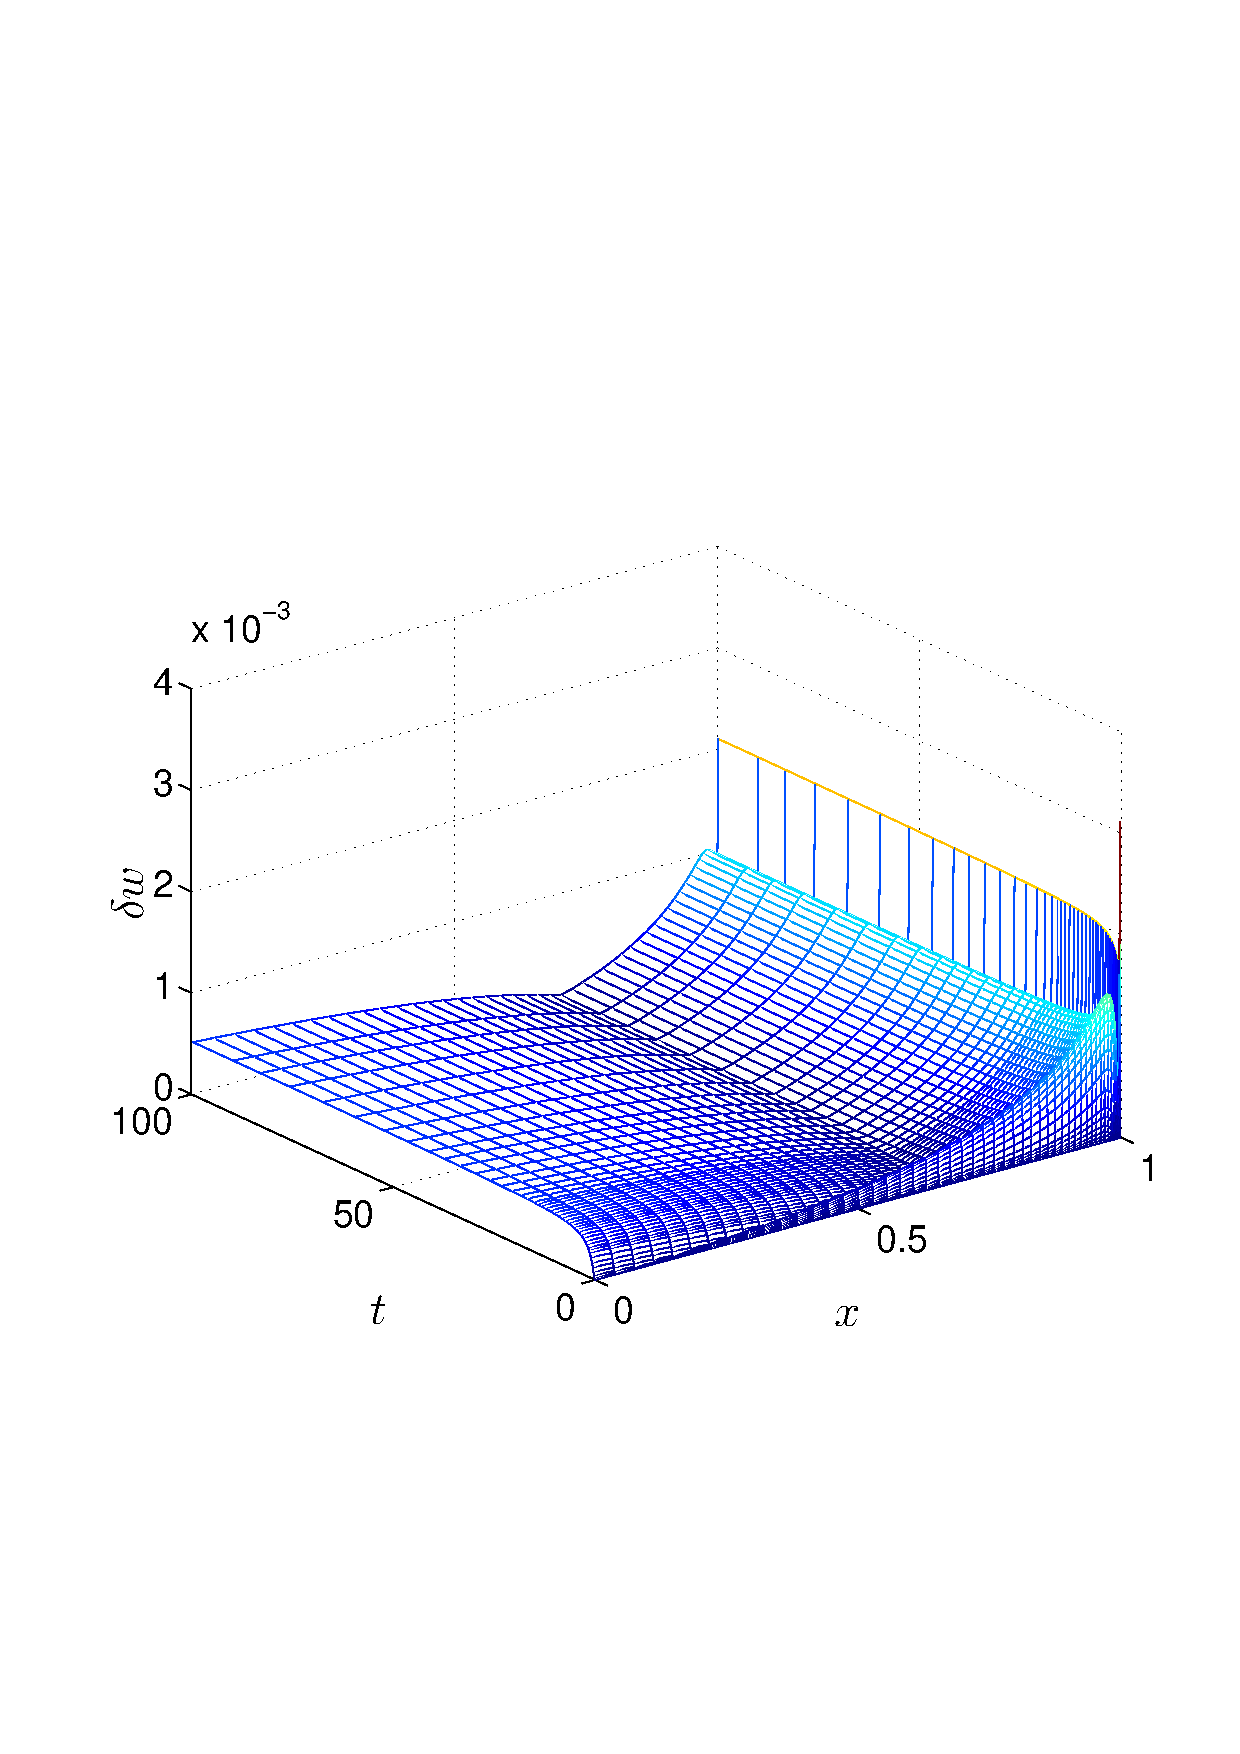
\includegraphics[width=\textwidth]{5_Multifracture_numerical/junction_test/standard_crack.png}
	\end{subfigure}
	\begin{subfigure}{0.45\textwidth}
		\centering
		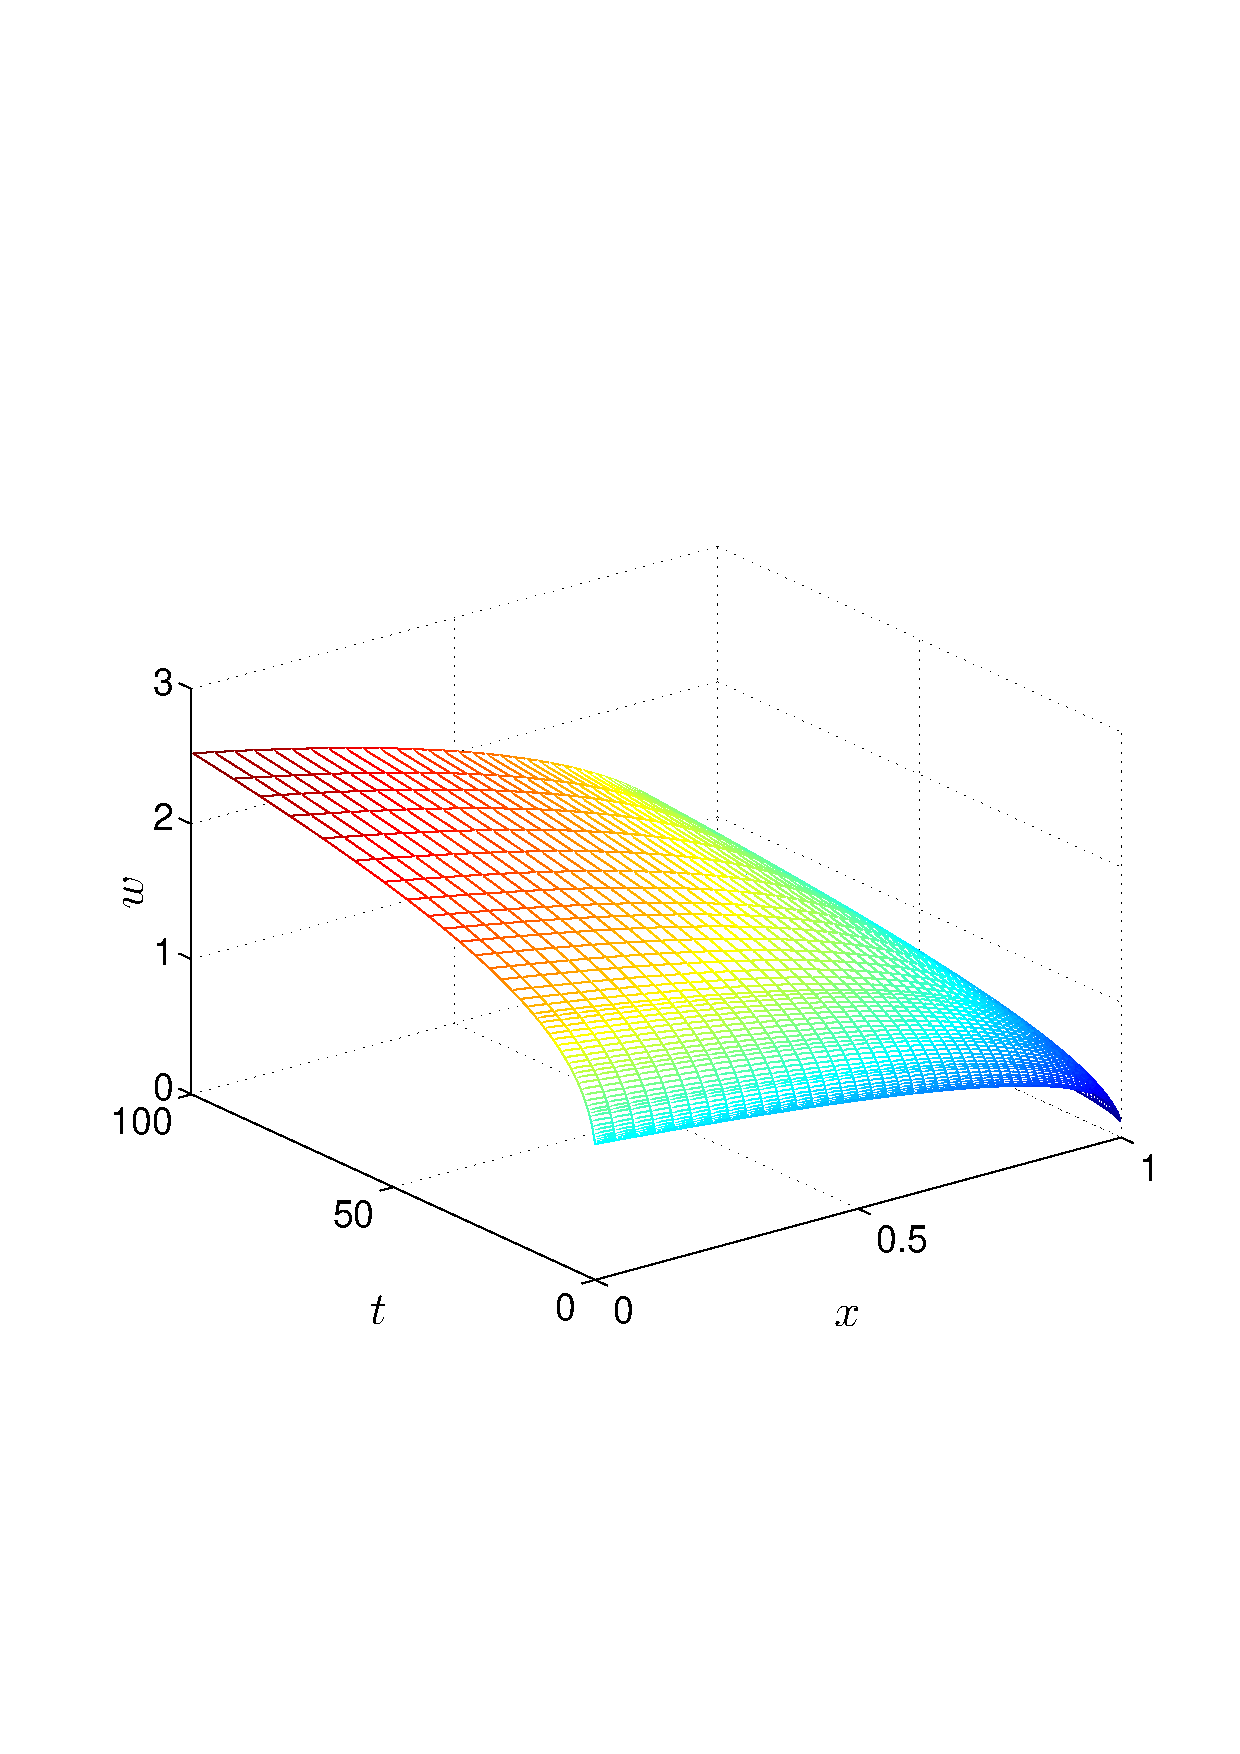
\includegraphics[width=\textwidth]{5_Multifracture_numerical/junction_test/standard_crack_sol.png}
	\end{subfigure}
	\caption{Relative error for for solving fracture with standard approach $\delta w_{max}=0.003120759916772$, and the actual fracture shape}
\end{figure}

\begin{figure}[H]
	\centering
	\begin{subfigure}{0.45\textwidth}
		\centering
		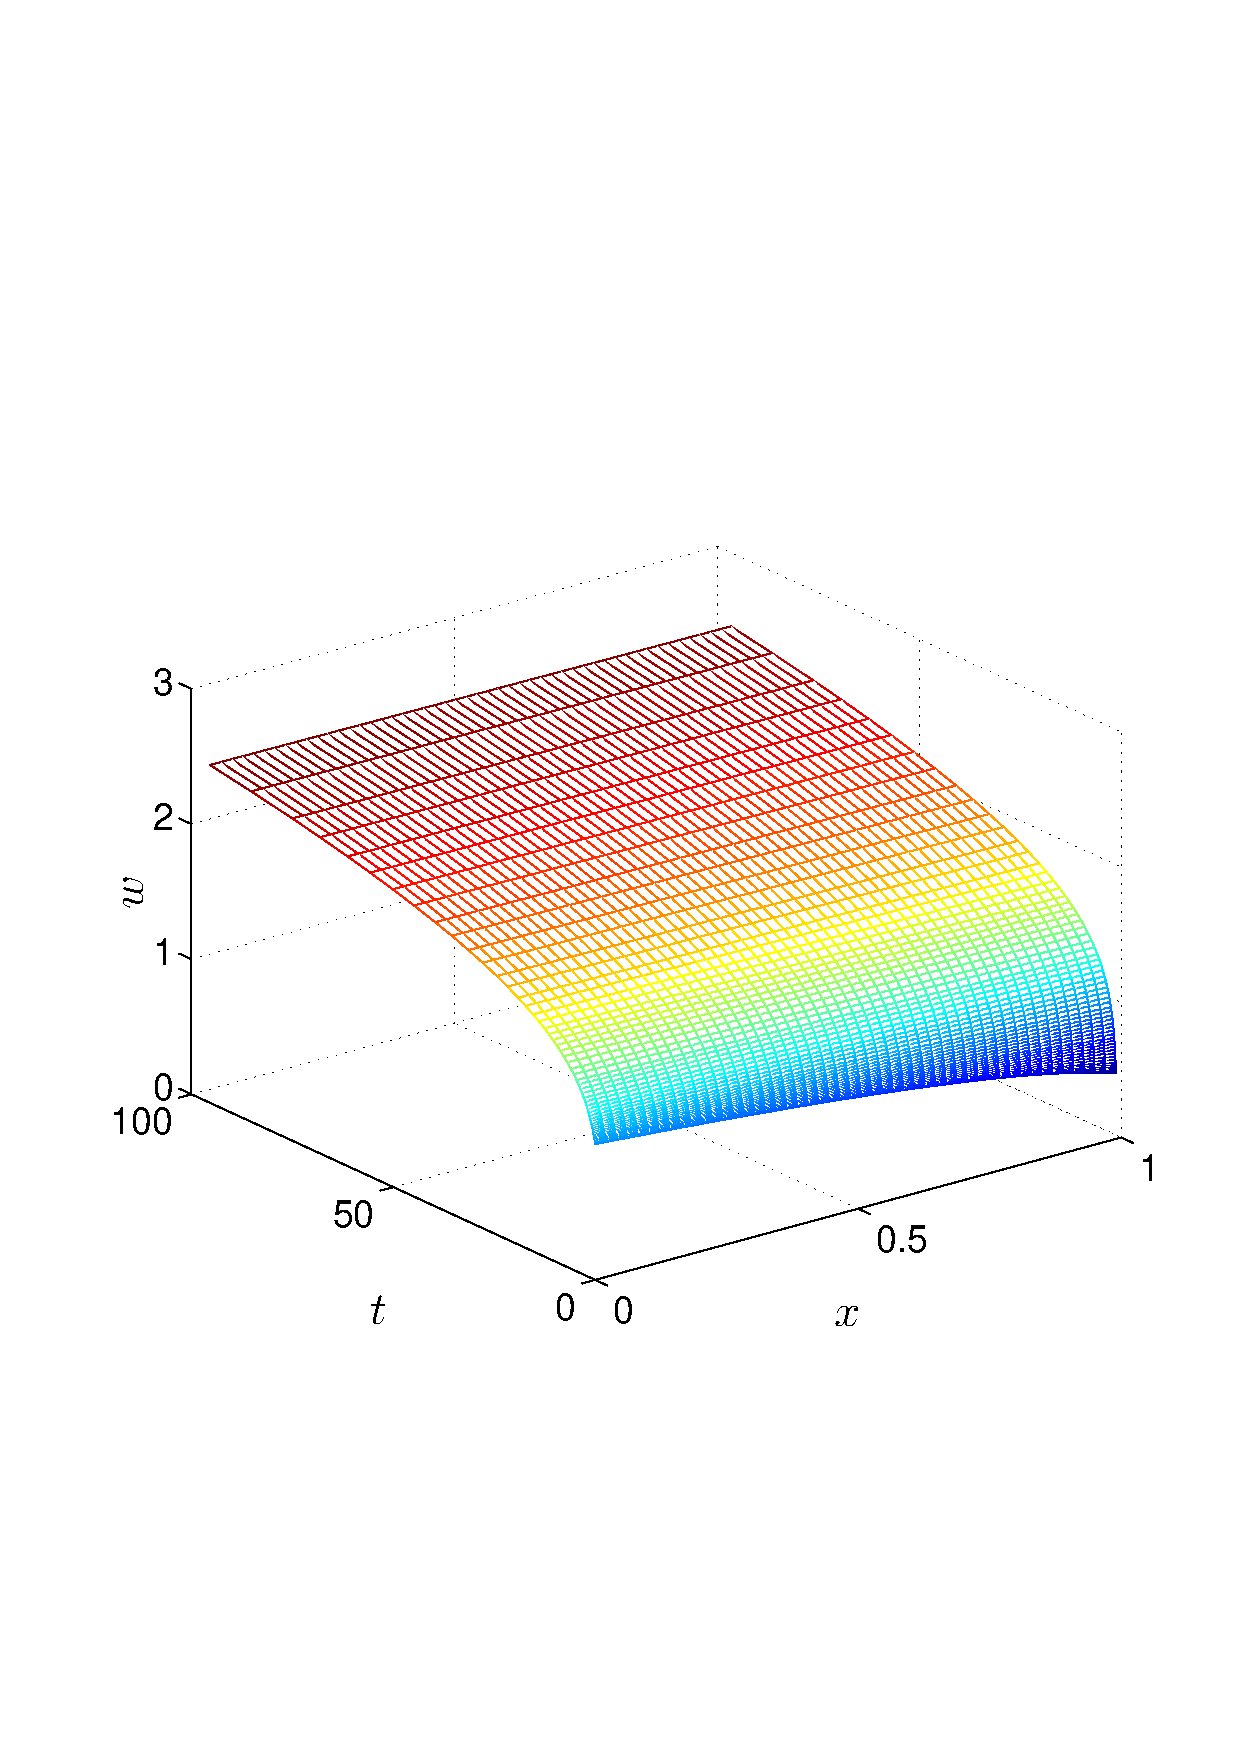
\includegraphics[width=\textwidth]{5_Multifracture_numerical/junction_test/pipe_sol.png}
	\end{subfigure}
	\begin{subfigure}{0.45\textwidth}
		\centering
		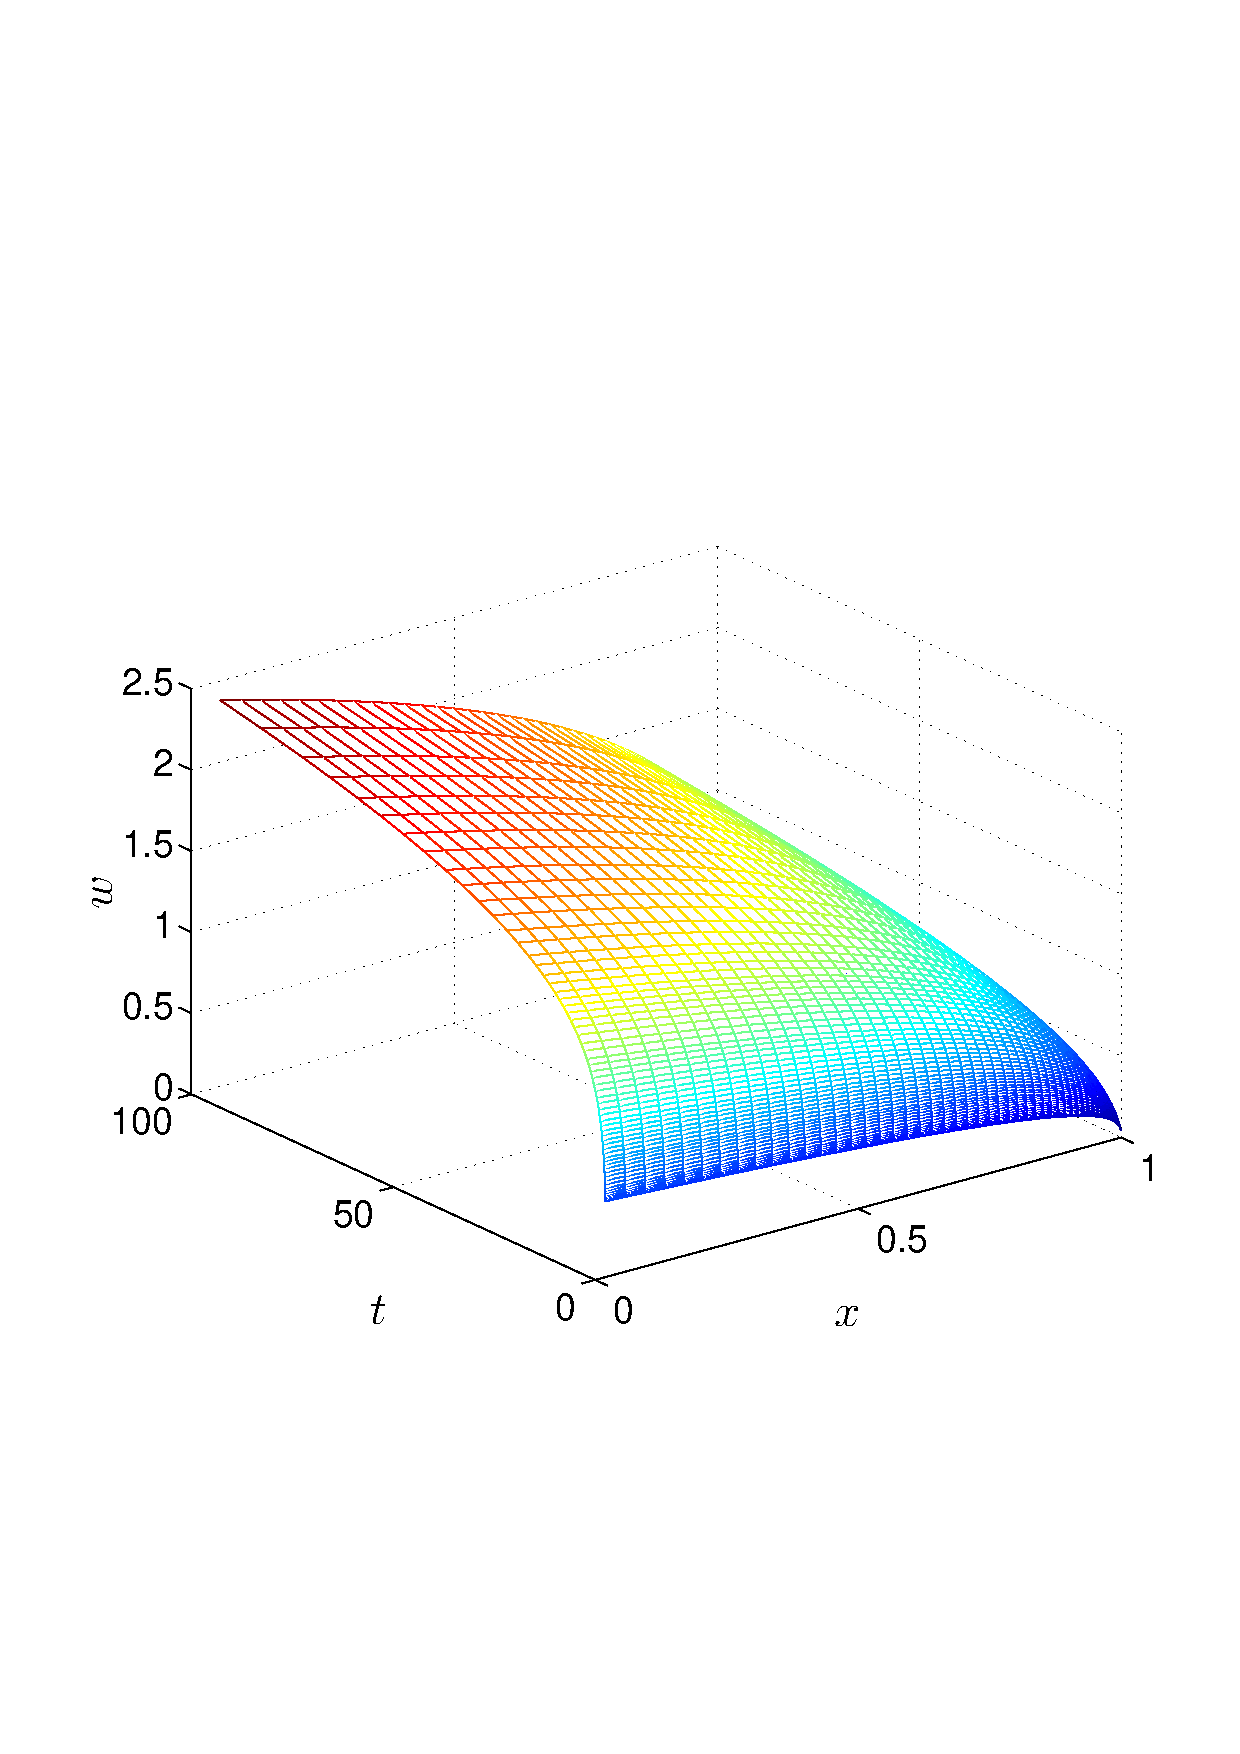
\includegraphics[width=\textwidth]{5_Multifracture_numerical/junction_test/crack_sol.png}
	\end{subfigure}
	\caption{The solutions split pipe and crack with $L_{split}=0.9$}
\end{figure}

\begin{figure}[H]
	\centering
	\begin{subfigure}{0.45\textwidth}
		\centering
		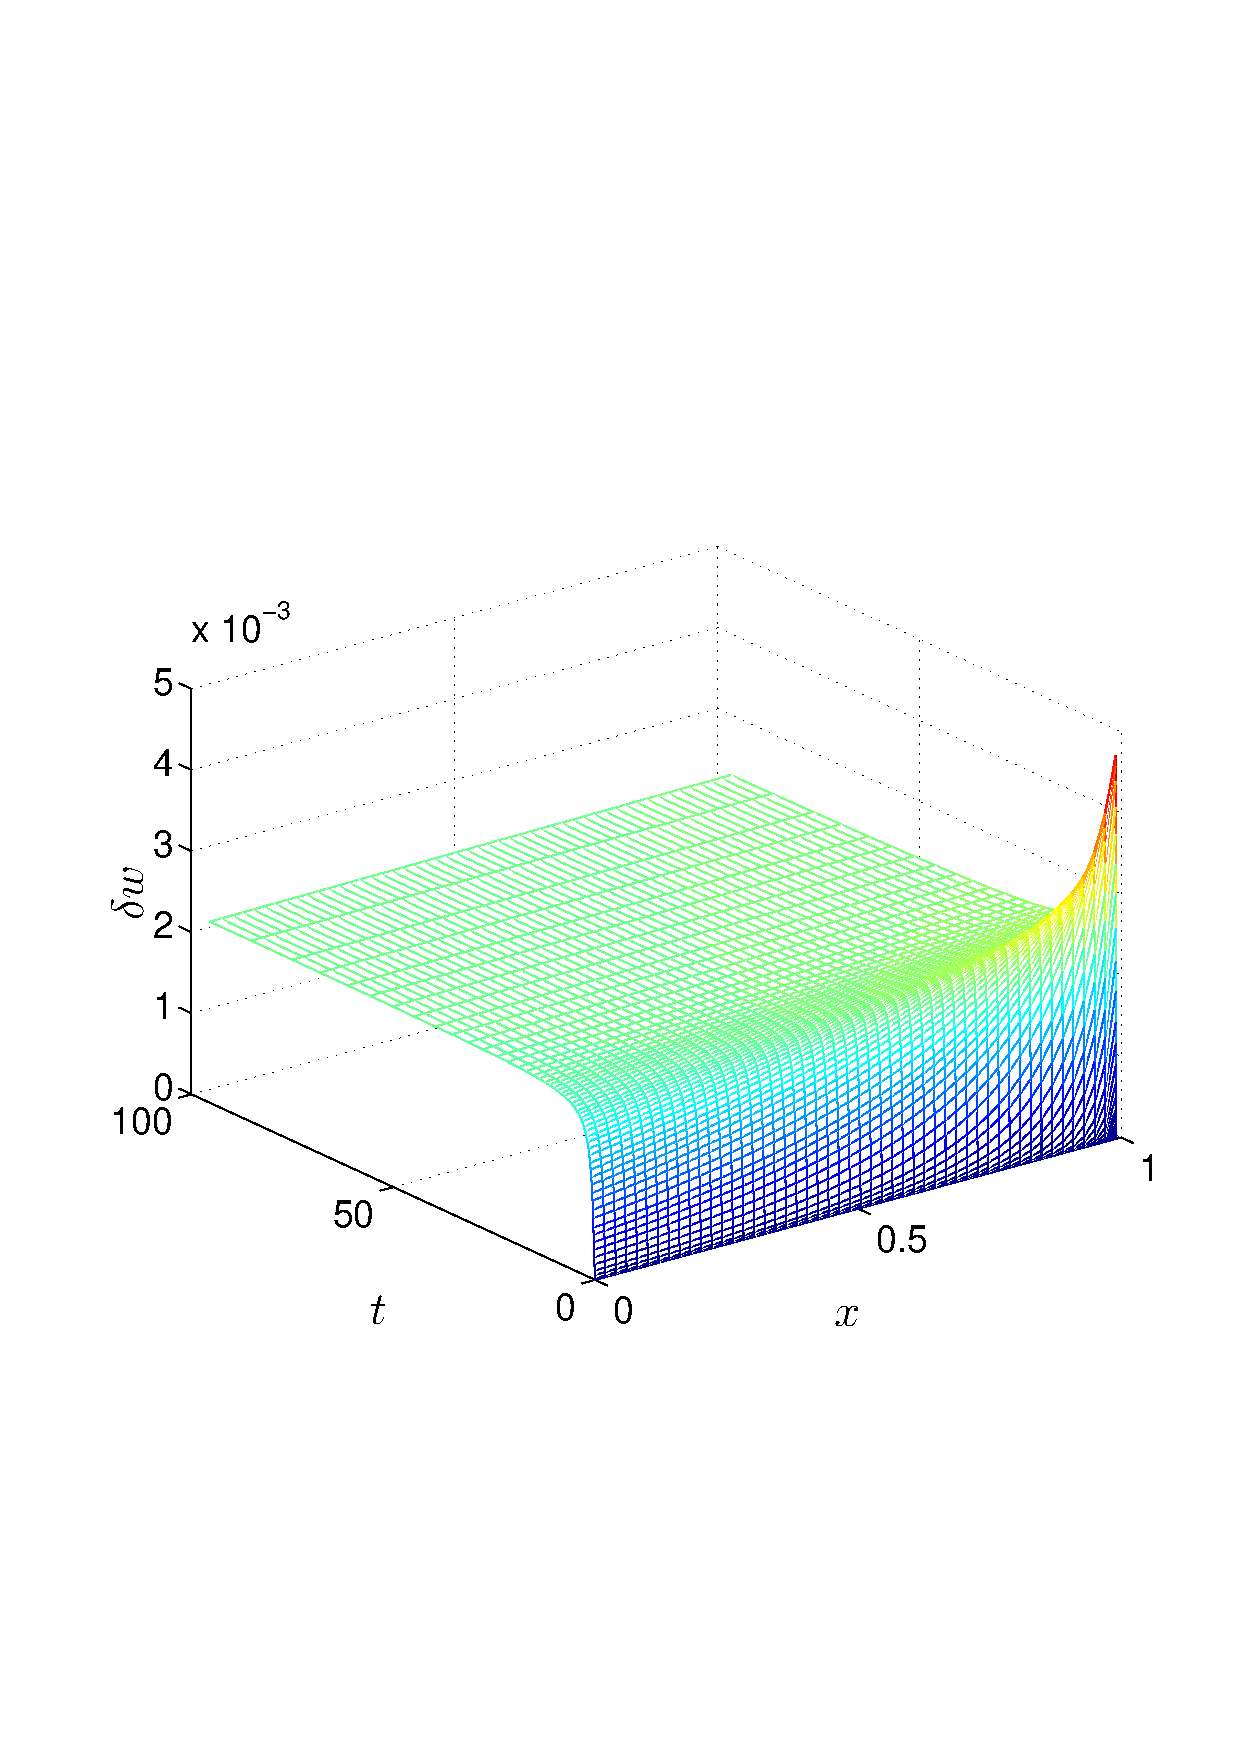
\includegraphics[width=\textwidth]{5_Multifracture_numerical/junction_test/lin_pipe_err.png}
	\end{subfigure}
	\begin{subfigure}{0.45\textwidth}
		\centering
		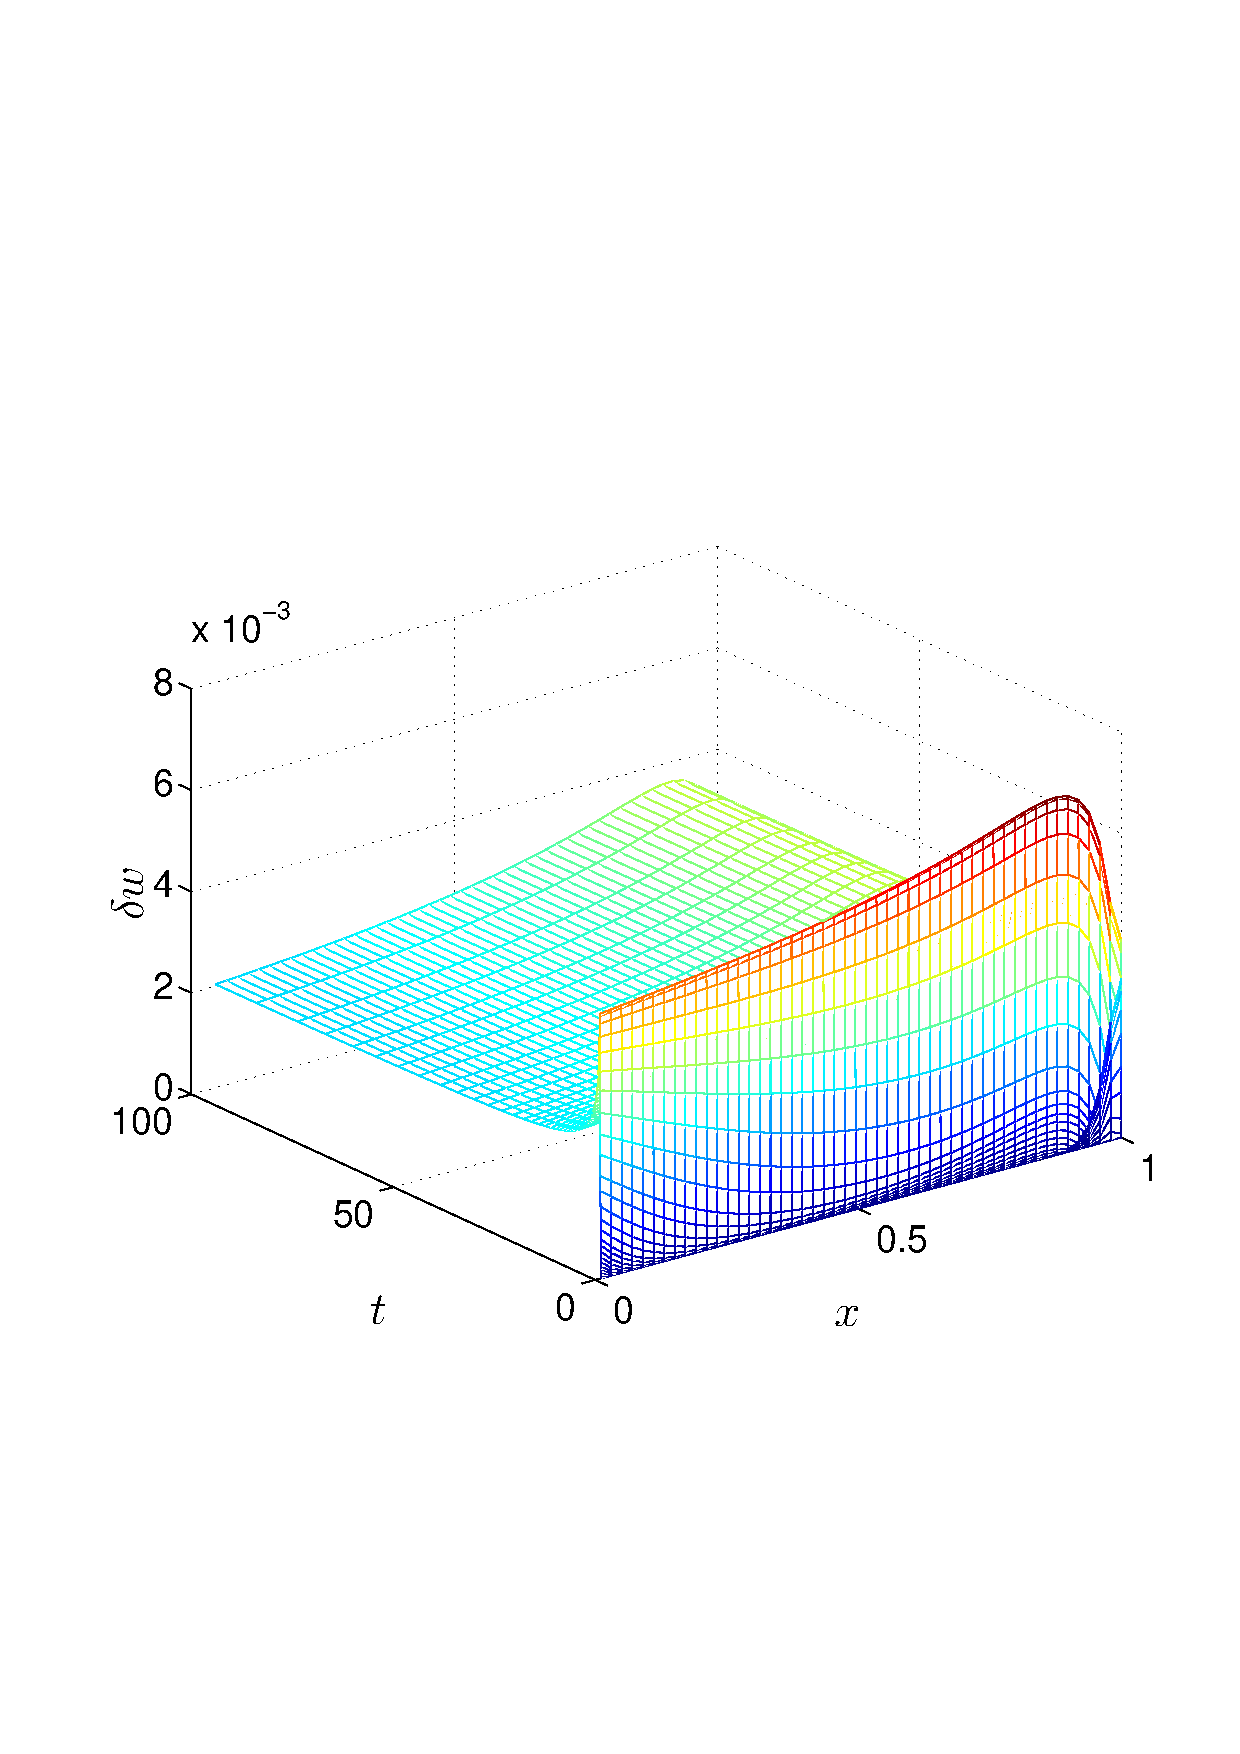
\includegraphics[width=\textwidth]{5_Multifracture_numerical/junction_test/lin_crack_err.png}
	\end{subfigure}
	\caption{Linear split $\delta w_{max}=0.007063202429168$}
\end{figure}

\begin{figure}[H]
	\centering
	\begin{subfigure}{0.45\textwidth}
		\centering
		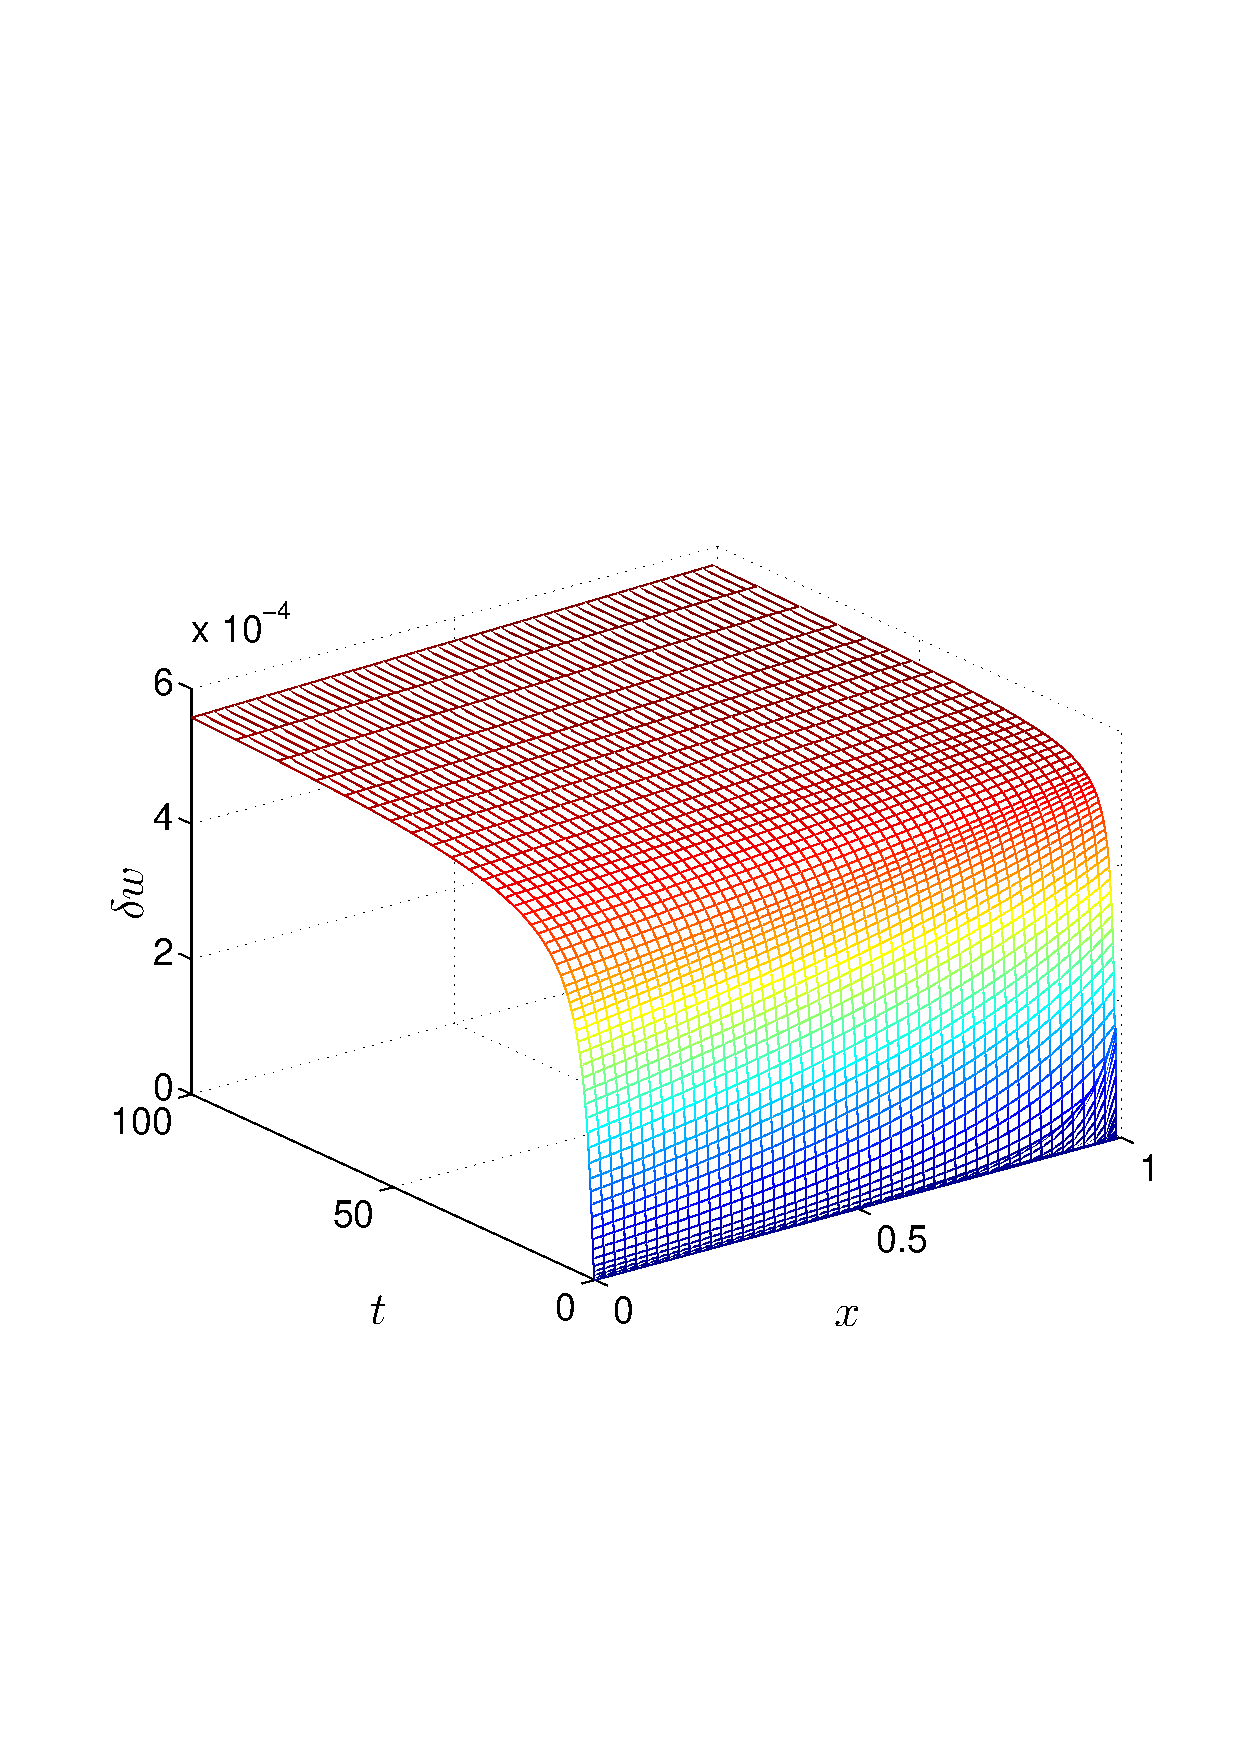
\includegraphics[width=\textwidth]{5_Multifracture_numerical/junction_test/quad_pipe_err.png}
	\end{subfigure}
	\begin{subfigure}{0.45\textwidth}
		\centering
		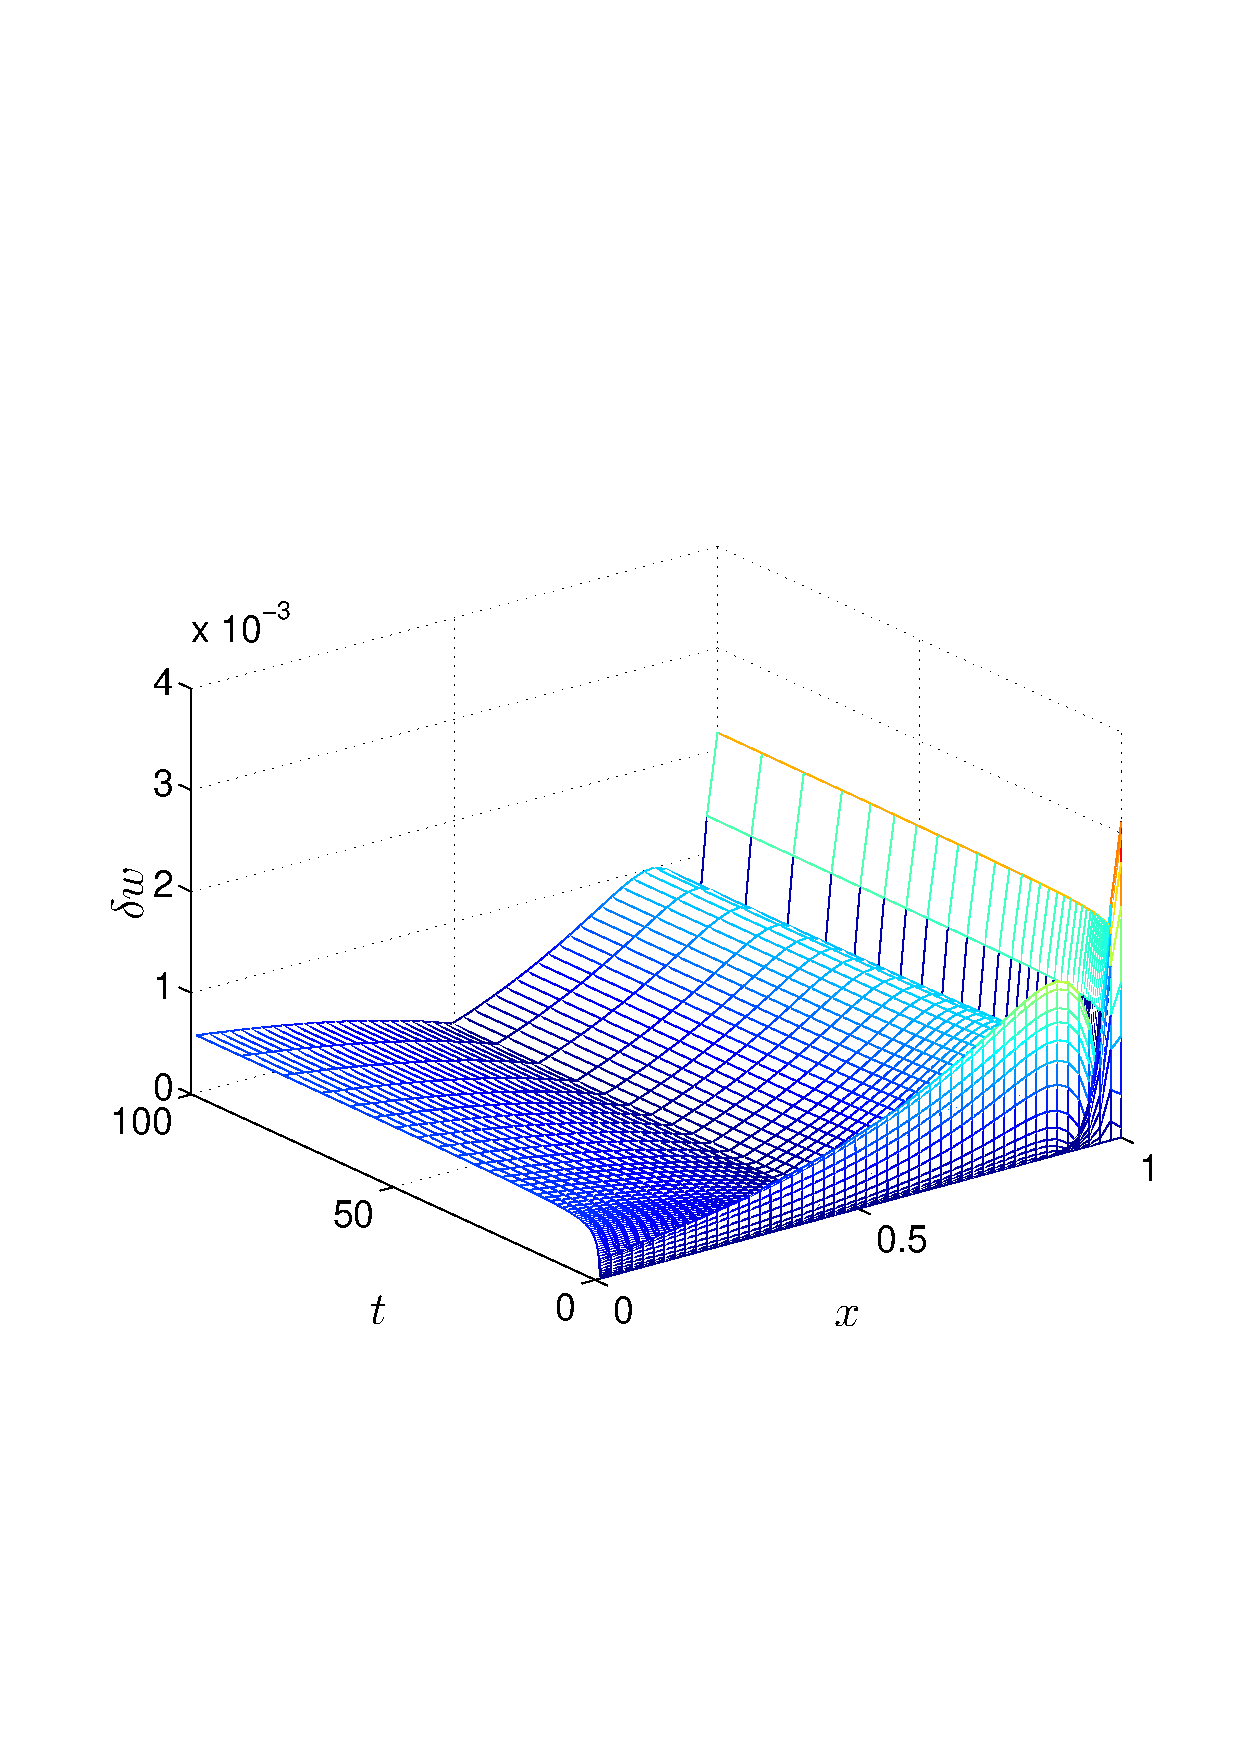
\includegraphics[width=\textwidth]{5_Multifracture_numerical/junction_test/quad_crack_err.png}
	\end{subfigure}
	\caption{Quadratic split $\delta w_{max}=0.003120504349734$}
\end{figure}


As we can see the linear fracture split condition works but adds some extra error, with magnitude twice the value when compared to standard computation. Both approaches however retain acceptable accuracy of the solution of order $10^{-3}$. The quadratic polynomial approach is however very close to producing identical error as the standard undivided solution. In fact the $\delta w_{max}$ is close that to the difference between these two is probably a result of the solver tolerance values. 
Conclusion, quadratic approximation allows to split fracture into segments without affecting computation accuracy.


\paragraph{finding accetable values of $L_{split}$ factor}

Lets make a test to find out what values of $L_{split}$ are acceptable.  Figure~\ref{L_split_large} shows that although the choice of $L_{split}$ has effect on accuracy, the fact that beginning crack can be of orders of magnitude shorter than pipe, indicates that attaching a small fracture to existing pipe should not cause significant lose in accuracy. Attaching a long fracture to some existing short pipe is on the other hand improbable scenario.

\begin{figure}[H]
	\centering
	\begin{subfigure}{0.45\textwidth}
		\centering
		\includegraphics[width=\textwidth]{5_Multifracture_numerical/junction_test/L_split.png}
	\end{subfigure}
	\begin{subfigure}{0.45\textwidth}
		\centering
		\includegraphics[width=\textwidth]{5_Multifracture_numerical/junction_test/L_split_small_crack.png}
	\end{subfigure}
	\caption{Testing how the different values of $L_{split}$ affects computational accuracy, in terms of fracture length, and with in pipe and crack segments. Close to $1$ values of $L_{split}$ generate large maximum error, however these values might be deceptive. Even with $L_split=1-10^{-9}$ solver eventually returns to normal accuracy in larger times, as showed by relative error in fracture length. $L_{split}$ values close to zero were however not possible to compute in feasible run time}
	\label{L_split_large}
\end{figure}


\paragraph{test with multiple segments in PKN fracture}

\begin{figure}[H]
  \centering
      \includegraphics[width=0.5\textwidth]{5_Multifracture_numerical/junction_test/p_p_p_crack}
  \caption{Tu obrazek z podzieleniem szczeliny na wiele segmentow z rura}
\end{figure}

Since quadratic split is obviously better than the linear split lets test it against more pipe segments crated in a single fracture. Again the precise benchmark was choosen, but this time more segments were allowed. The results are presented in the figure below \ref{L_segments} :

\begin{figure}[H]
	\centering
	\includegraphics[width=\textwidth]{5_Multifracture_numerical/junction_test/segment_test.png}
	\caption{Error in $\delta L$ for various numbers off segments splits with different $N$ points for pipe and crack segments. Interestingly accuracy is only relay by the number of grid points in new crack segment. The number of pipe segments can be as much one hundred with only $10$ points per pipe, but the accuracy remains unchanged.}
	\label{L_segments}
\end{figure}
 




